\documentclass[compress]{beamer}        % [compress] (written before {beamer} <=> navigation bar one line, all subsections in 1 line instead of 2

% Setup appearance:
\usetheme{CambridgeUS}
%	AnnArbor | Antibes | Bergen |
%	Berkeley | Berlin | Boadilla |
%	boxes | CambridgeUS | Copenhagen |
%	Darmstadt | default | Dresden |
%	Frankfurt | Goettingen |Hannover |
%	Ilmenau | JuanLesPins | Luebeck |
%	Madrid | Malmoe | Marburg |
%	Montpellier | PaloAlto | Pittsburgh |
%	Rochester | Singapore | Szeged |
%	Warsaw
%

\useoutertheme[footline=authorinstitute,subsection=false]{miniframes}
\usecolortheme{whale}

%	albatross | beaver | beetle |
%	crane | default | dolphin |
%	dove | fly | lily | orchid |
%	rose |seagull | seahorse |
%	sidebartab | structure |
%	whale | wolverine


\setbeamertemplate{footline}
{
  \hbox{%
  \begin{beamercolorbox}[wd=.25\paperwidth,ht=2.25ex,dp=1ex,center]{title in head/foot}%
    \usebeamerfont{date in head/foot}\insertshortauthor
  \end{beamercolorbox}%
  \begin{beamercolorbox}[wd=.5\paperwidth,ht=2.25ex,dp=1ex,center]{date in head/foot}%
    \usebeamerfont{title in head/foot}\insertshortinstitute
  \end{beamercolorbox}%
  \begin{beamercolorbox}[wd=.25\paperwidth,ht=2.25ex,dp=1ex,center]{title in head/foot}%
    \usebeamerfont{date in head/foot}
    \insertframenumber{} / \inserttotalframenumber
    %\insertframenumber{} / \insertpresentationendpage
  \end{beamercolorbox}}%
  \vskip0pt%
}

%\setbeamercolor{titlelike}{parent=structure}
%\setbeamercolor{structure}{fg=beamer@blendedblue}
%% \useinnertheme{rounded}
%\setbeamerfont{block title}{size={}}
%\usefonttheme[onlylarge]{structurebold}   % title and words in the table of contents bold
%\setbeamerfont*{frametitle}{size=\normalsize,series=\bfseries}
\setbeamertemplate{navigation symbols}{}
\setbeamercolor{frametitle}{parent=boxes, bg=white}
{ % only on titlepage


\usepackage{times}
\usepackage{amsmath,amssymb,amsthm}
\usepackage{color}
\usepackage{changepage}
\usepackage{multirow}
\usepackage[absolute,overlay]{textpos}
\usepackage{enumerate}
%\usepackage{pgfpages}
\usepackage[all]{xy}
\usepackage{textcomp}
\usepackage{etex}
\usepackage{tikz}
\usetikzlibrary{shapes}
%\usepackage{handoutWithNotes}
%\pgfpagesuselayout{4 on 1}[border shrink=1mm]




\definecolor{camblue}{RGB}{26,26,89}
\definecolor{Rblue}{RGB}{0,255,255}
\definecolor{Rdarkblue}{RGB}{0,0,255}
\definecolor{Rgreen}{RGB}{0,205,0}
\definecolor{green2}{RGB}{51,204,51}
\newcommand{\tcb}{\textcolor{beamer@blendedblue}}
\newcommand{\tcbb}{\textcolor{camblue}}
\newcommand{\tcr}{\textcolor{red}}
\newcommand{\tcg}{\textcolor{gray}}
\newcommand{\tcgr}{\textcolor{green2}}
\newcommand{\tcblk}{\textcolor{black}}
\newcommand{\tcRg}{\textcolor{Rgreen}}
\newcommand{\tcRdb}{\textcolor{Rdarkblue}}
\newcommand{\tcRb}{\textcolor{Rblue}}
\newcommand{\tcw}{\textcolor{white}}
\newcommand{\m}{\phantom{-}}
\newcommand{\bp}{\tcbb{$\bullet$}\:}


\title{{\huge Statistics for Computing\\[0.1cm]MA4413}}
\author[Kevin Burke]{{\bf\\[0.5cm]{\huge Lecture 2}\\[0.2cm]\emph{Numerical Summaries of Centrality and Dispersion and the Boxplot}\\[1.4cm]Kevin Burke}\\[0.3cm]\tcb{kevin.burke@ul.ie}}

\institute[University of Limerick, Maths \& Stats Dept]{}
\date{}

%\TPGrid[5mm,5mm]{1}{1}

\begin{document}


\begin{frame}[t]
\titlepage
\end{frame}


\section{Numerical Summaries}
\subsection{Numerical Summaries}
\begin{frame}{\bf \tcb{Numerical Summaries}}
We focus here on \emph{numerical data} only. We have seen how the frequency table and corresponding histogram describe the whole distribution of data.\\[0.4cm]
Often however, we would like to summarise the {\bf main features} of the distribution without using the whole frequency table, i.e., a few numbers - \emph{``numerical summaries''} - which provide the relevant info.\\[0.5cm]
We will look at measures of:
\begin{itemize}\itemsep0.4cm
\item {\bf Centrality} - a numeric value indicating the centre of the distribution, i.e., an ``average'' or ``typical'' value.
\item {\bf Dispersion} - a numeric value indicating the degree to which measurements \emph{vary} about this centre, i.e., is the distribution of values tightly packed around its centre or not?
\end{itemize}

\end{frame}

\subsection{Numerical Summaries}
\begin{frame}{\bf \tcb{Numerical Summaries}\\[-1cm]}
\begin{itemize}\itemsep0.3cm
\item {\bf Centrality}
\begin{itemize}\itemsep0.2cm
\item mean: arithmetic average (you all know this).
\item median: middle number in the \emph{ordered} data.
\end{itemize}
\item {\bf Dispersion}
\begin{itemize}\itemsep0.2cm
\item range: $\max(x) -\min(x)$.
\item variance: measure of variation around the \emph{mean}.
\item standard deviation: square root of the variance.
\item quartiles: \emph{three} numbers - $Q_1$,$Q_2$ and $Q_3$ - which split the \emph{ordered}\newline\phantom{quartiles:} data into four parts (note: $Q_2 =$ the median).
\item inter-quartile range: $IQR = Q_3 - Q_1$.\\[0.4cm]
\end{itemize}
\end{itemize}
We also introduce the {\bf boxplot} - a graphical method for numerical data. This could have gone into the ``Visualising Numerical Data'' section of Lecture 1 but we need $Q_1$,$Q_2$, $Q_3$ and $IQR$ to draw it.
\end{frame}


\section{Centrality}
\subsection{The Mean}
\begin{frame}{\bf \tcb{The Mean}}
The mean is just the usual arithmetic average: add all of the individual data values in the sample and divide by the number of values.\\[0.5cm]
Remember that {\boldmath$n$} is the symbol for the \emph{sample size}, i.e., the number of values. The sample mean is:\\[-0.6cm]

\begin{align*}
\boxed{\bar x = \frac{x_1 + x_2 + \ldots + x_n}{n} = \frac{\sum x_i}{n}}.
\end{align*}

We have introduced the \emph{sum notation} - don't be put off by this! $\sum$ just means ``the sum of'' and $x_i$ means ``individual value''. So $\sum x_i$ means ``the sum of all values''.\\[0.4cm]
Remember that we have seen the symbol $\bar x$ before. Also, recall that it is a \emph{statistic} which \emph{estimates} the population mean $\mu$ \emph{(parameter)}.

\end{frame}

\subsection{The Mean: Example}
\begin{frame}{\bf \tcb{The Mean: Example}}
Let's say we have the annual income (in thousands) of $n = 5$ individuals living in a particular apartment block:
\begin{center}
\begin{tabular}{|ccccc|}
\hline
&&&&\\[-0.4cm]
25 & 29 & 33 & 35 & 40 \\
\hline
\multicolumn{5}{c}{}\\
\end{tabular}
\end{center}
The average income is
\begin{align*}
\bar x = \frac{25 + 29 + 33 + 35 + 40}{5} &= \frac{162}{5} \\[0.2cm]
&= 32.4 \\[0.2cm]
&= \text{\texteuro\,} 32,400.
\end{align*}


\end{frame}



\subsection{The Mean - Skewed Data}
\begin{frame}{\bf \tcb{The Mean - Skewed Data}}
An issue with the mean is its sensitivity to \emph{outliers} - data values much larger / smaller than the main body of data - which lead to \emph{skewness} (remember: data can be skewed to the right / left).\\[0.4cm]
Let's now assume that the 5th individual is \emph{much} wealthier than the others:
\begin{center}
\begin{tabular}{|ccccc|}
\hline
&&&&\\[-0.4cm]
25 & 29 & 33 & 35 & 500 \\
\hline
\multicolumn{5}{c}{}\\
\end{tabular}
\end{center}
The average income is
\begin{align*}
\bar x = \frac{25 + 29 + 33 + 35 + 500}{5} &= \frac{622}{5} \\[0.2cm]
&= 124.4 \\[0.2cm]
&= \text{\texteuro\,} 124,400.
\end{align*}


\end{frame}


\subsection{The Mean - Skewed Data}
\begin{frame}{\bf \tcb{The Mean - Skewed Data}}

It is clear that \texteuro\,124,400 is not a good representation of the centre of the income distribution. It is not a typical income for an individual living in that apartment block.\\[0.6cm]

The mean gets \emph{pulled towards} the outliers, i.e., it is pulled away from the centre in the direction of the skew.\\[0.3cm]
\begin{itemize}\itemsep0.5cm
\item Data skewed to the right (caused by large values) \newline\phantom{\quad}$\Rightarrow$ the mean gets pulled towards the right.\\[0.4cm]
\item Data skewed to the left (caused by small values) \newline\phantom{\quad}$\Rightarrow$ the mean gets pulled towards the left.
\end{itemize}

\end{frame}




\subsection{The Median}
\begin{frame}{\bf \tcb{The Median}}
The median, $Q_2$, is the value that splits the \emph{ordered} data in half:\\
50\% of the data lies above $Q_2$ and 50\% of the data lies below it.\\
{\footnotesize(Note: we call the median $Q_2$ as it is the second quartile - more on this later)}\\[0.6cm]

To find $Q_2$:\\[0.2cm]
\begin{enumerate}[1.]\itemsep0.4cm
\item Put the data \emph{in order} - smallest to largest - if it is not already.
\item $Q_2$ is then the value in \emph{position} $\boxed{\frac{n+1}{2}}$ where $n$ is the sample size.\\[0.6cm]
\end{enumerate}

{\bf Important}: $\tfrac{n+1}{2}$ is not the value of the median, it is its \emph{position} in the\newline\phantom{{\bf Important}:} ordered data.

\end{frame}


\subsection{The Median: Example}
\begin{frame}{\bf \tcb{The Median: Example}\\[-1.1cm]}
\begin{adjustwidth}{-1.5cm}{}
\begin{center}
\begin{tabular}{r|ccccc|}
\multicolumn{1}{c}{} & \multicolumn{5}{c}{\emph{Position}} \\
\multicolumn{1}{c}{} & \emph{1}  & \emph{2}  & \emph{\tcr{3}}  & \emph{4}  & \multicolumn{1}{c}{\emph{5}} \\
\cline{2-6}
&&&&&\\[-0.4cm]
{\bf Symmetrical}: & 25 & 29 & \tcb{33} & 35 & 40 \\
\cline{2-6}
\multicolumn{6}{c}{}\\
\cline{2-6}
&&&&&\\[-0.4cm]
{\bf Skewed to the Right}: & 25 & 29 & \tcb{33} & 35 & 500 \\
\cline{2-6}
\multicolumn{6}{c}{}\\[0.4cm]
\end{tabular}
\end{center}
\end{adjustwidth}
The \emph{\tcr{position}} of the median is:
\begin{align*}
\frac{n+1}{2} = \frac{5+1}{2} = \frac{6}{2} = \tcr{3},\\[-0.6cm]
\end{align*}
i.e., the \tcr{3rd} number.\\[0.4cm]

$\Rightarrow$ The \emph{\tcb{value}} is:\,\, $Q_2 = \tcb{33} = \text{\texteuro}\,33,000$.\\[0.4cm]

The median is unaffected by skewness - it still gives an accurate estimate of the centre.

\end{frame}


\subsection{Mean Vs Median}
\begin{frame}{\bf \tcb{Mean Vs Median}\\[-1.3cm]}
\begin{columns}

\begin{column}{.5\textwidth}
\begin{adjustwidth}{-0.1cm}{0.0cm}
\begin{itemize}\itemsep2.3cm
\item Symmetrical data: $\tcr{\bar x} \approx \tcRg{Q_2}$.
\item Right-skewed: $\tcr{\bar x} > \tcRg{Q_2}$.
\item Left-skewed: $\tcr{\bar x} < \tcRg{Q_2}$.
\end{itemize}
\end{adjustwidth}
\end{column}

\begin{column}{.5\textwidth}
\begin{adjustwidth}{-0.3cm}{0.0cm}

\begin{tabular}{c}
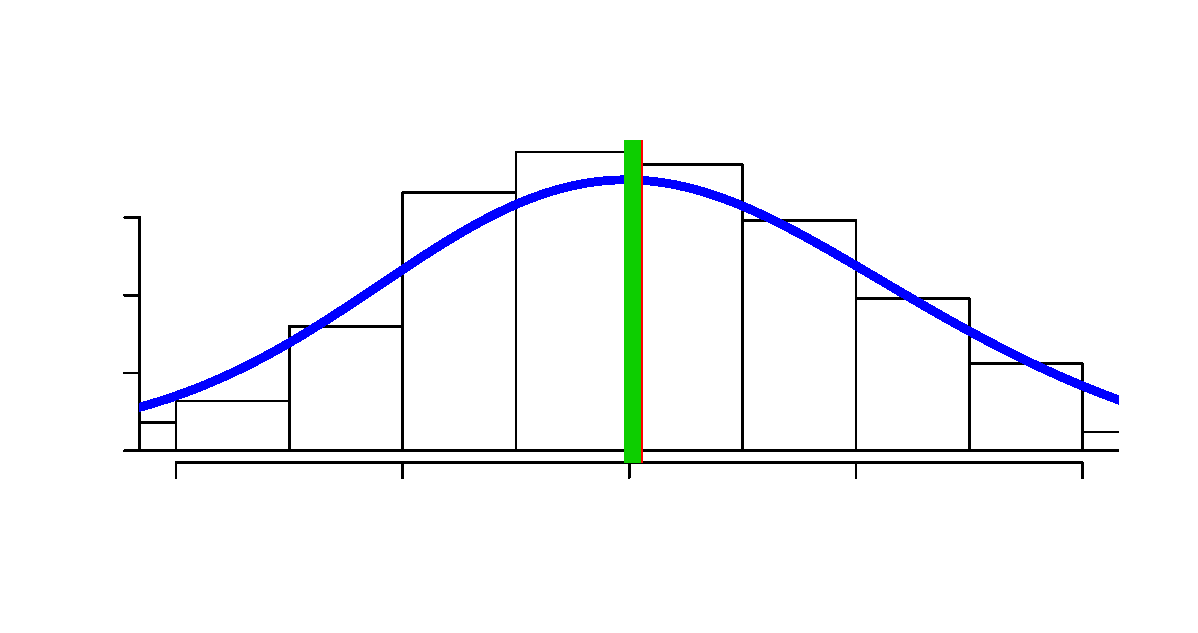
\includegraphics[width=1\textwidth, trim = 0.0cm 0.5cm 0.3cm 1.5cm, clip]{Symmetrical2}\\
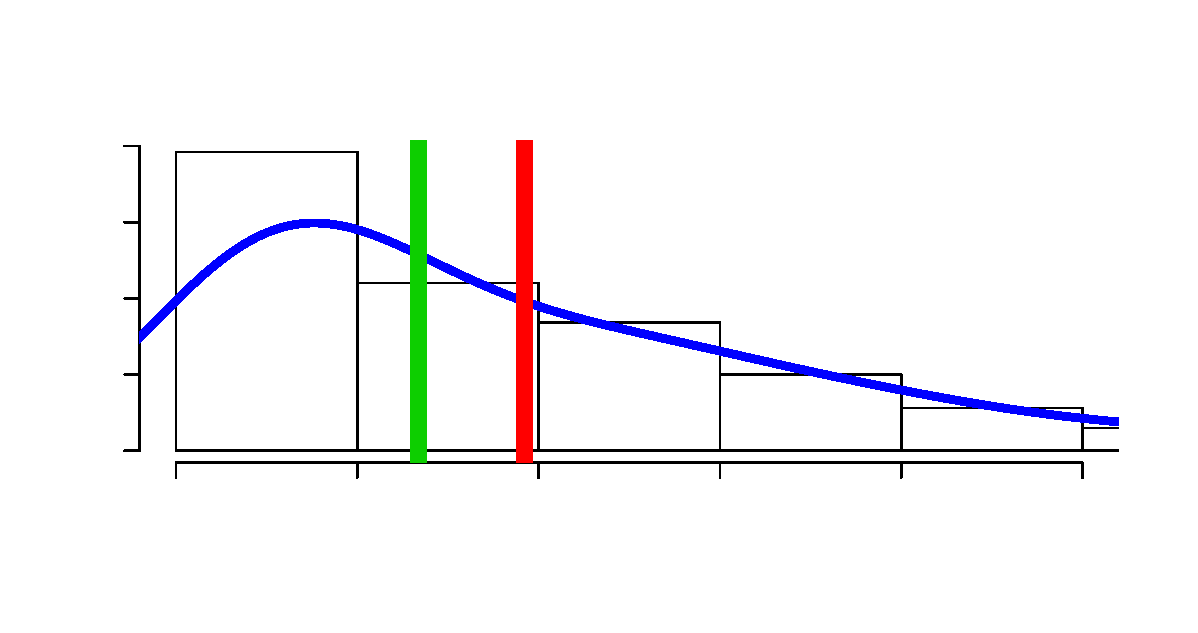
\includegraphics[width=1\textwidth, trim = 0.0cm 0.5cm 0.3cm 1.5cm, clip]{SkewRight2}\\
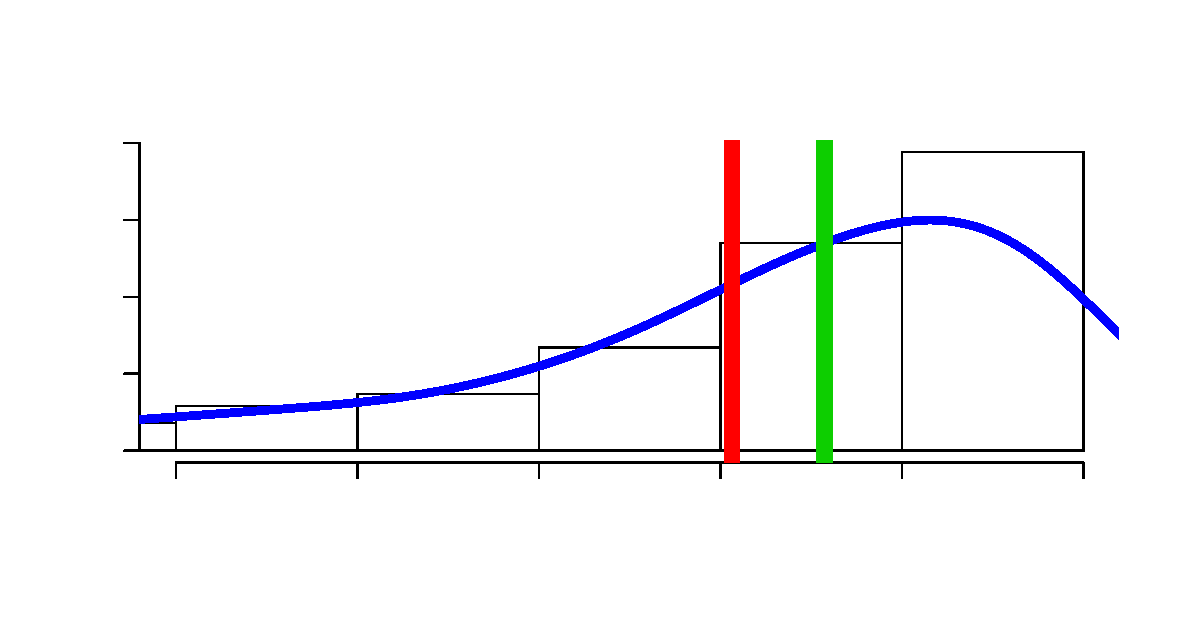
\includegraphics[width=1\textwidth, trim = 0.0cm 0.5cm 0.3cm 1.5cm, clip]{SkewLeft2}
\end{tabular}


\end{adjustwidth}
\end{column}

\end{columns}

\end{frame}


\subsection{The Median: There's No Middle of 6 Numbers!}
\begin{frame}{\bf \tcb{The Median: There's No Middle of 6 Numbers!}}

Let's say we have 6 numbers - what is the median?

\begin{center}
\begin{tabular}{|cccccc|}
\multicolumn{6}{c}{\emph{Position}} \\
\multicolumn{1}{c}{\emph{1}} & \emph{2}  & \emph{\tcr{3}}  & \emph{\tcr{4}}  & \emph{5}  & \multicolumn{1}{c}{\emph{6}} \\
\hline
&&&&&\\[-0.4cm]
10 & 13 & 15 & 21 & 32 & 42 \\
\hline
\multicolumn{6}{c}{}\\[-0.3cm]
\end{tabular}
\end{center}
The \emph{\tcr{position}} of the median is:
\begin{align*}
\frac{n+1}{2} = \frac{6+1}{2} = \frac{7}{2} = \tcr{3.5},\\[-0.6cm]
\end{align*}
i.e., the median lies \emph{between} the \tcr{3rd} and \tcr{4th} numbers.\\[0.5cm]

$\Rightarrow$ Its \emph{\tcb{value}} is simply the \emph{average} of the numbers in position \tcr{3} and \tcr{4}:
\begin{equation*}
Q_2 = \tfrac{15+21}{2} = \tfrac{36}{2} = \tcb{18}.
\end{equation*}

\end{frame}


\subsection{Question 1}
\begin{frame}{\bf \tcb{Question 1}\\[-0.8cm]}
Consider the following \emph{sample} of numbers:
\begin{center}
\begin{tabular}{|cccccccccc|}
\hline
&&&&&&&&&\\[-0.4cm]
2 & 4 & 2 & 1 & 5 & 3 & 0 & 4 & 1 & 8 \\
\hline
\end{tabular}
\end{center}
\begin{enumerate}[a)]\itemsep0.3cm
\item What is the value of $n$\,?
\item Calculate the mean and use the appropriate symbol.
\item What is the symbol for the population mean? What is its value?
\item Calculate $Q_2$ (hint: need to order the data first).
\item Construct a frequency table with 3 classes (let zero be the first breakpoint).
\item Draw the corresponding histogram.
\end{enumerate}
\end{frame}



\section{Dispersion\hspace{0.9cm}}
\subsection{Dispersion}
\begin{frame}{\bf \tcb{Dispersion}}
The centre of the distribution is only part of the story. We also need to know how spread out - \emph{dispersed} - the data values are.\\[0.8cm]

Consider the following:\\[0.4cm]

A software engineer is offered a job with an annual salary of \texteuro\,45,000. The employer says that this is a very attractive salary as it is above the average for this type of job (\texteuro\,40,000).\\[0.4cm]
Is this a good offer?... We don't know. Not without knowing how much the data \emph{varies} about the central value.
\end{frame}


\subsection{Dispersion}
\begin{frame}{\bf \tcb{Dispersion}\\[-1.2cm]}
\begin{center}
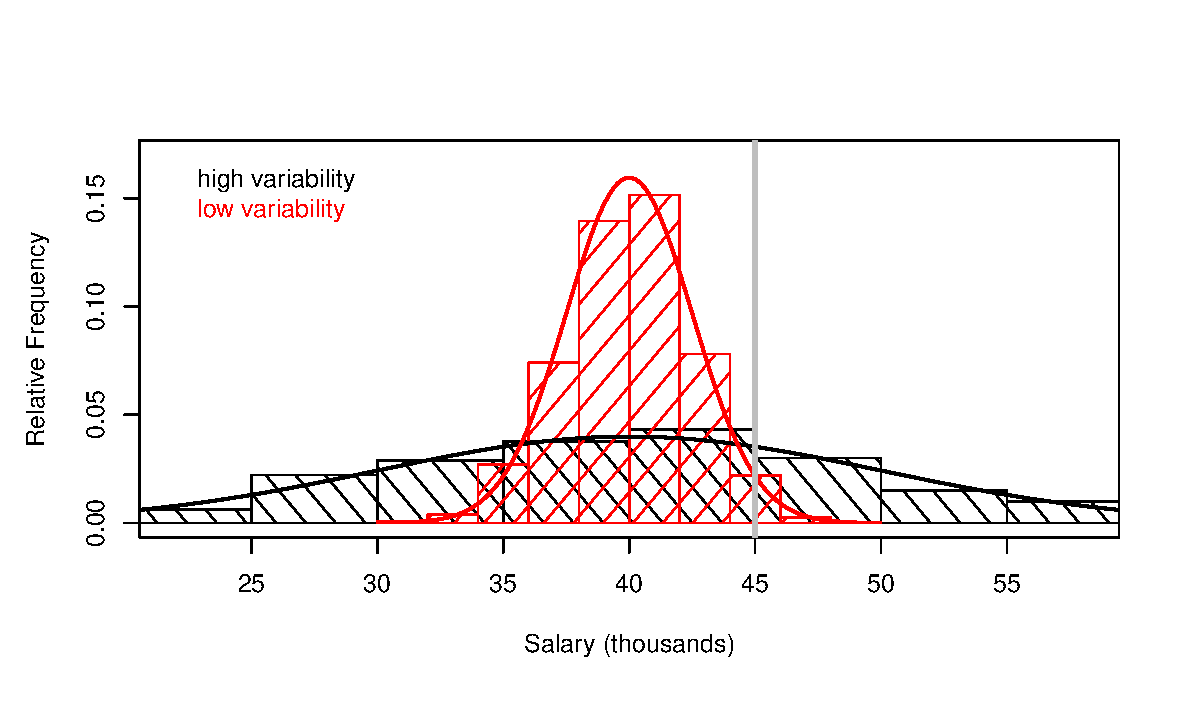
\includegraphics[width=1\textwidth, trim = 0.0cm 0.6cm 0.3cm 1.5cm, clip]{Variance}
\end{center}
\vspace{-0.1cm}
If the distribution of salaries is highly variable, there are many posts available with a better salary. On the other hand, if variability is very low, we have been offered one of the highest salaries in the field.
\end{frame}


\subsection{The Range}
\begin{frame}{\bf \tcb{The Range}}

The most basic measure of dispersion is the {\bf range} of the data.\\[-0.4cm]

\begin{align*}
\boxed{\text{range} = \max(x) - \min(x)},
\end{align*}
i.e., the largest value minus the smallest value in the set of data.\\[0.8cm]

Disadvantage: It only tells us the \emph{overall spread} of the data. But what we really want to know is how the data varies about its centre.\\[0.5cm]

We mainly focus on other techniques (standard deviation and inter-quartile range).

\end{frame}


\subsection{The Variance}
\begin{frame}{\bf \tcb{The Variance}}
The {\bf variance} is the \emph{average squared distance from the mean} and is given by:\\[-0.6cm]
\begin{align*}
s^2 &= \frac{(x_1 - \bar x)^2 + (x_2 - \bar x)^2 + \ldots + (x_n - \bar x)^2}{n-1}\\[0.2cm]
&= \frac{\sum (x_i - \bar x)^2}{n-1}
\end{align*}
In words, subtract the mean from each value, square the results and then add them all together. Finally, divide by $n-1$.\\
{\footnotesize(For technical reasons, in the case of variance, we divide by $n-1$ rather than $n$)}\\[0.7cm]
The units of variance are \emph{squared-units}, for example, if we were looking at income (in euro) then the variance would be in euros-squared.

%You might wonder why we divide by $n-1$ instead of $n$ as in the case of the mean. The theory behind this is beyond the scope of this course but it turns out that dividing by $n-1$ is the correct approach for the variance.

\end{frame}

\subsection{The Variance}
\begin{frame}{\bf \tcb{The Variance}}
It turns out that the previous formula can be rewritten as:\\
{\footnotesize(if you're good with sums, i.e., $\Sigma$, then you can show this)}\\[0.2cm]
\begin{align*}
\boxed{s^2 = \frac{\sum x_i^2 - n\,{\bar x}^2}{n-1}}\\
\end{align*}
This version of the formula involves less computation so we will use it.\\[0.5cm]


\end{frame}

\subsection{The Standard Deviation}
\begin{frame}{\bf \tcb{The Standard Deviation}}
The {\bf standard deviation} is a \emph{very} important quantity in statistics (as we will see later in this course).\\[0.5cm]

The standard deviation is the \emph{square root} of the variance:
\begin{align*}
\boxed{s = \sqrt{s^2} = \sqrt{\frac{\sum x_i^2 - n\,{\bar x}^2}{n-1}}}.\\
\end{align*}
Since the variance is in squared-units, the standard deviation has \emph{the same units as the data} (as a result of taking the square root).

\end{frame}


\subsection{The Standard Deviation: Example}
\begin{frame}{\bf \tcb{The Standard Deviation: Example}}
We return to our earlier example - the incomes of 5 individuals. \\[0.3cm]

\begin{center}
\begin{tabular}{|c@{\hspace{0.3cm}}|ccccc|c@{\hspace{0.1cm}}c|}
 \multicolumn{6}{c}{} && \multicolumn{1}{c}{$\sum$} \\[0.2cm]
\hline
&&&&&&&\\[-0.4cm]
$x_i$ & 25 & 29 & 33 & 35 & 40 && 162 \\[0.1cm]
\hline
&&&&&&&\\[-0.3cm]
$x_i^2$ & 625 & 841 & 1089 & 1225 & 1600 && 5380 \\[0.1cm]
\hline
\multicolumn{8}{c}{}\\[-0.4cm]
\end{tabular}
\end{center}

Using the above and the mean value, $\bar x = \tfrac{162}{5} = 32.4$, we then calculate the variance:\\[-0.3cm]
\begin{align*}
s^2 = \frac{\sum x_i^2 - n\,{\bar x}^2}{n-1} = \frac{5380 - 5 \, (32.4^2)}{5-1} &= \frac{5380 - 5 \, (1049.76)}{4} \\[0.1cm]
&= \frac{5380 - 524.8}{4} \\[0.1cm]
&= \frac{131.2}{4} = 32.8 = 32,800 \, \text{\texteuro$^2$}.
\end{align*}

\end{frame}


\subsection{The Standard Deviation: Example}
\begin{frame}{\bf \tcb{The Standard Deviation: Example}}

The standard deviation is then

\begin{align*}
s = \sqrt{s^2} = \sqrt{32.8} = 5.727 = 5,727 \, \text{\texteuro}.\\
\end{align*}

{\bf Note the units are euros}.

\end{frame}


\subsection{Symbols}
\begin{frame}{\bf \tcb{Symbols}}
It is worth preparing ourselves for things to come:\\[0.4cm]

\begin{itemize}\itemsep0.4cm
\item For the \emph{sample standard deviation} we use the symbol $s$ as shown.
\item For the true \emph{population standard deviation} we use $\sigma$ (the Greek letter ``sigma'').\\[0.6cm]
\end{itemize}

Naturally we have $s^2$ and $\sigma^2$ for the sample variance and population variance.\\[0.8cm]

Don't forget, sample \emph{statistics} estimate the true population \emph{parameters}.

\end{frame}


\subsection{Important Note on Dispersion Measures}
\begin{frame}{\bf \tcb{Important Note on Dispersion Measures}}

Variance and standard deviation are {\bf\emph{always positive numbers}}.\\[0.7cm]

In fact \emph{all} measures of dispersion are positive numbers.\\[1.8cm]

Consider the following four  numbers: \boxed{-10,\,\,-9,\,\,-5,\,\,-4}.\\[0.3cm] Clearly the centre is negative; however, standard deviation will not be. Show that $\bar x = -7$ and $s = 2.94$.

\end{frame}



\subsection{Question 2}
\begin{frame}{\bf \tcb{Question 2}}
25 individuals were asked how long their laptop lasts on a full charge. The recorded times (measured in hours) are as follows:\\
{\footnotesize(we saw this dataset before - lecture 1, Q5)}
\begin{center}
\begin{tabular}{|cccccccccc|}
\hline
&&&&&&&&&\\[-0.4cm]
2.2 & 0.4 & 4.2 & 12.9 & 1.5 & 3.0 & 5.7  & 0.7 & 1.0 & 3.3 \\
0.2 & 0.2 & 5.6 &  1.6 & 3.0 & 0.1 & 14.3 & 3.4 & 0.9 & 6.1 \\
1.4 & 1.0 & 0.7 & 5.4  & 2.3 &&&&&\\
\hline
\end{tabular}
\end{center}
\begin{enumerate}[a)]\itemsep0.3cm
\item Calculate $\bar x$.
\item Calculate $s$.
\item What is the symbol for the population standard deviation? What is our best estimate of this?
\item What is the value of $\mu$?
\item What is the value of $\hat p$?
\end{enumerate}
\end{frame}

\subsection{The Standard Deviation - Skewed Data}
\begin{frame}{\bf \tcb{The Standard Deviation - Skewed Data}}

Recall that $\bar x$ is \emph{not} a good measure of centrality when data is skewed (use the median, $Q_2$, instead).\\[0.6cm]
If this is the case, we are then not interested in $s$\, either since this measures the dispersion about $\bar x$.\\[1cm]
So what goes with the median? - The \emph{inter-quartile range}.


\end{frame}


\subsection{Quartiles}
\begin{frame}{\bf \tcb{Quartiles}}

There are {\bf three quartiles} which split the (ordered!) data into four parts:\\[-0.4cm]
\begin{align*}
25\% - {\bf Q_1} - 25\% - {\bf Q_2} - 25\% - {\bf Q_3} - 25\%
\end{align*}
The process of finding the quartiles is essentially the same as the case of finding the median (i.e., the second quartile $Q_2$).\\[0.4cm]
\begin{enumerate}[1.]
\item Put the data \emph{in order} - smallest to largest.
\item The \emph{position} of $Q_k$ (quartile number $k$) is:
    \boxed{\frac{n+1}{4}\times k}.\\[0.6cm]
\end{enumerate}

$Q_1$ is in position $\tfrac{n+1}{4}$, $Q_2$ is in position $\tfrac{n+1}{4}\times2$ and $Q_3$ is in position $\tfrac{n+1}{4}\times3$.

\end{frame}


\subsection{The Inter-Quartile Range}
\begin{frame}{\bf \tcb{Inter-Quartile Range}}

The {\bf inter-quartile range} is the range of the middle 50\% of data.\\[1.2cm]

Calculation of IQR is straightforward once we have the quartiles:
\begin{align*}
\boxed{IQR = Q_3 - Q_1},\\[-0.1cm]
\end{align*}
i.e., it is simply the difference between the upper and lower quartiles.

\end{frame}




\subsection{Quartiles and IQR: Example}
\begin{frame}{\bf \tcb{Quartiles and IQR: Example}}
Consider the following sample of $n=10$ values:\\[-0.2cm]
\begin{center}
\begin{tabular}{|cccccccccc|}
\hline
&&&&&&&&&\\[-0.4cm]
2 & 4 & 2 & 1 & 5 & 3 & 0 & 4 & 1 & 8 \\
\hline
\end{tabular}
\end{center}
First we must \emph{sort} the values. The reordered dataset is:\\[-0.2cm]
\begin{center}
\begin{tabular}{|ccccccccccc|}
\multicolumn{1}{c}{\emph{Positions:}} & \multicolumn{1}{c}{\emph{1}} & \emph{\tcr{2}} & \emph{\tcr{3}} & \emph{4} & \emph{\tcb{5}} & \emph{\tcb{6}} & \emph{7} & \emph{\tcRg{8}} & \emph{\tcRg{9}} & \multicolumn{1}{c}{\emph{10}} \\
\cline{1-11}
&&&&&&&&&&\\[-0.4cm]
\multicolumn{1}{|c}{\emph{Values:}} & 0 & 1 & 1 & 2 & 2 & 3 & 4 & 4 & 5 & 8 \\
\cline{1-11}
\end{tabular}
\end{center}


\begin{tabular}{c|c|c}
{\bf Quartile} & {\bf Position} & {\bf Value} \\[0.1cm]
$Q_1$ & $\tfrac{10+1}{4} = \tfrac{11}{4} = 2.75$\,\,$\Rightarrow$ between \tcr{2} \& \tcr{3} & $\tfrac{1+1}{2} = {\bf1}$\\[0.3cm]
$Q_2$ & $\tfrac{11}{4}\times2 = 2.75\times2 = 5.5$\,\,$\Rightarrow$ between \tcb{5} \& \tcb{6} & $\tfrac{2+3}{2} = {\bf2.5}$\\[0.3cm]
$Q_3$ & $\tfrac{11}{4}\times3 = 2.75\times3 = 8.25$ $\Rightarrow$ between \tcRg{8} \& \tcRg{9} & $\tfrac{4+5}{2} = {\bf4.5}$\\
\multicolumn{3}{c}{}\\
\end{tabular}

$\Rightarrow$ {\bf IQR} $= Q_3 - Q_1 = 4.5 - 1 = {\bf3.5}$. \\
{\footnotesize (3.5 units covers the middle 50\% of data)}

\end{frame}


\subsection{Question 3}
\begin{frame}{\bf \tcb{Question 3}}
We return to the laptop battery life data:\\
\begin{center}
\begin{tabular}{|cccccccccc|}
\hline
&&&&&&&&&\\[-0.4cm]
2.2 & 0.4 & 4.2 & 12.9 & 1.5 & 3.0 & 5.7  & 0.7 & 1.0 & 3.3 \\
0.2 & 0.2 & 5.6 &  1.6 & 3.0 & 0.1 & 14.3 & 3.4 & 0.9 & 6.1 \\
1.4 & 1.0 & 0.7 & 5.4  & 2.3 &&&&&\\
\hline
\end{tabular}
\end{center}
\begin{enumerate}[a)]\itemsep0.3cm
\item What is the value of $n$\,?
\item Find the values of the quartiles.
\item Calculate IQR.
\item Calculate $\bar x$ and compare this to $Q_2$. Is the data skewed? If so, in what direction?
\end{enumerate}
\end{frame}



\section{Boxplot}
\subsection{Boxplot}
\begin{frame}{\bf \tcb{Boxplot}}
A {\bf boxplot} is a graph containing the following items:\\[0.3cm]
\begin{enumerate}[1.]\itemsep0.6cm
\item Quartiles: $Q_1$, $Q_2$ and $Q_3$.
\item Mimimum/maximum values \emph{not classed as outliers}.
\item Outliers (values much smaller/larger than the main body of data).\\[1cm]
\end{enumerate}

We know how to get quartiles. All we need to know is how to classify data as being outliers.

\end{frame}


\subsection{Outlier Detection}
\begin{frame}{\bf \tcb{Outlier Detection}}

To find outliers we first calculate the {\bf lower fence} and {\bf upper fence}:
\begin{center}
\begin{tabular}{|c|}
\hline
\\[-0.4cm]
$LF = Q_1 - 1.5 \times IQR$ \\[0.2cm]
$UF = Q_3 + 1.5 \times IQR$ \\
\hline
\end{tabular}
\end{center}

\begin{itemize}
\item {\bf Outliers} are then:\\[0.2cm]
\begin{itemize}\itemsep0.4cm
\item Values smaller than LF.
\item Values greater than UF.
\end{itemize}
\end{itemize}


\end{frame}


\subsection{Outlier Detection: Example}
\begin{frame}{\bf \tcb{Outlier Detection: Example}}

Let's look at the laptop battery data. In Question 3 we should have found that $Q_1 = 0.8$, $Q_2 = 2.2$, $Q_3 = 4.8$ and $IQR = 4$.\\[0.3cm]

So we have
\begin{align*}
LF &= Q_1 - 1.5 \times IQR\\
   &= 0.8 - 1.5 \times 4 = -5.2. \\[0.3cm]
UF &= Q_3 + 1.5 \times IQR\\
   &= 4.8 + 1.5 \times 4 = \m10.8. \\
\end{align*}

Any value in the data less than -5.2 or greater than 10.8 is classed as an outlier.

\end{frame}


\subsection{Outlier Detection: Example}
\begin{frame}{\bf \tcb{Outlier Detection: Example}}
Looking at the \emph{ordered} data:
\begin{center}
\begin{tabular}{|cccccccccc|}
\hline
&&&&&&&&&\\[-0.4cm]
0.1 & 0.2 & 0.2 & 0.4 & 0.7 & 0.7 & 0.9 & 1.0  & 1.0 & 1.4 \\
1.5 & 1.6 & 2.2 & 2.3 & 3.0 & 3.0 & 3.3 & 3.4 & 4.2 & 5.4  \\
5.6 & 5.7 & 6.1 & 12.9 & 14.3 &&&&&\\
\hline
\end{tabular}
\end{center}

\begin{itemize}
\item Values less than $LF = - 5.2$:\quad {\bf none}.
\item Values greater than $UF = 10.8$:\quad {\bf 12.9 and 14.3}.\\[0.3cm]
\item Minimum of non-outliers: {\bf 0.1}.
\item Maximum of non outliers: {\bf 6.1}.\\[0.5cm]
\end{itemize}

\emph{We can now draw the boxplot}.

\end{frame}



\subsection{Boxplot: Example}
\begin{frame}{\bf \tcb{Boxplot: Example}\\[-1.1cm]}
\begin{center}
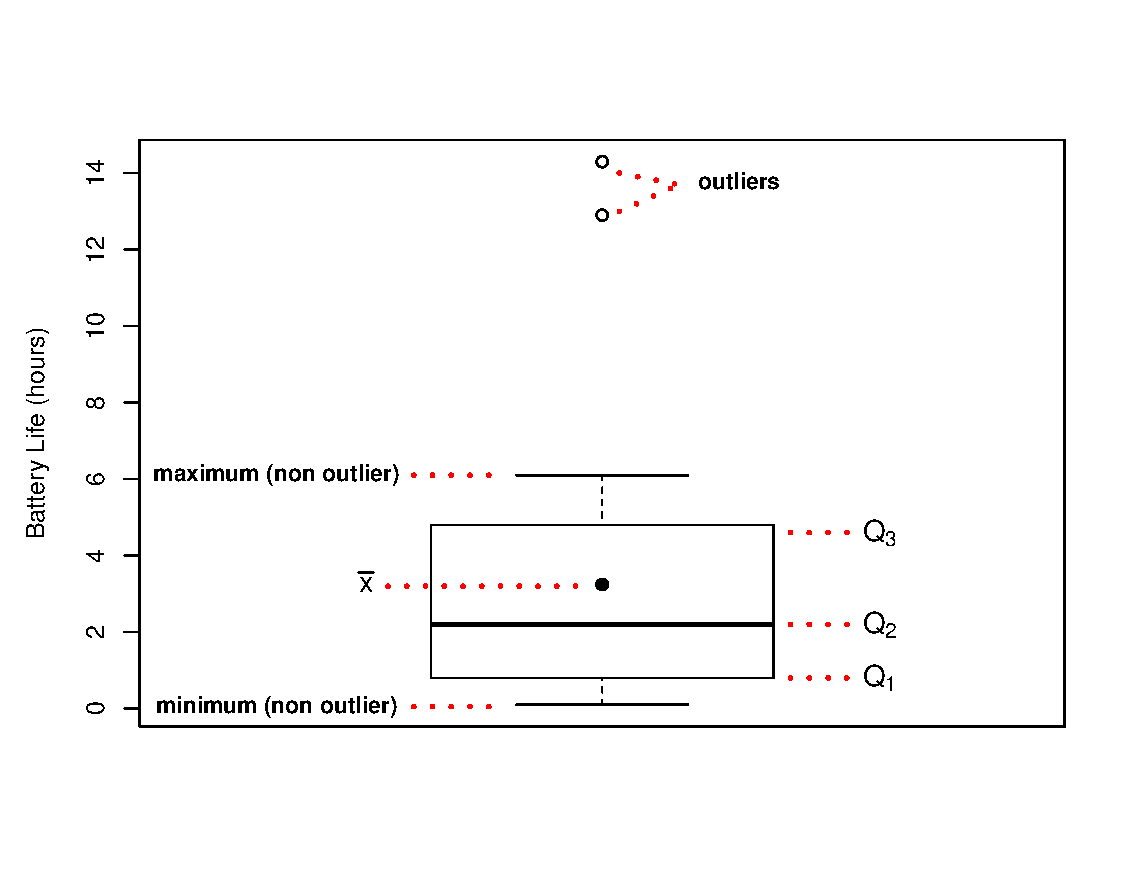
\includegraphics[width=0.8\textwidth, trim = 0.0cm 0.5cm 0.3cm 1cm, clip]{BoxplotLabelled}
\end{center}
\begin{itemize}\itemsep0.2cm
\item Labelled boxplot. Note - it is also useful to include $\bar x$.
\end{itemize}

\end{frame}


\subsection{Boxplot: Example}
\begin{frame}{\bf \tcb{Boxplot: Example}\\[-1.1cm]}
\begin{center}
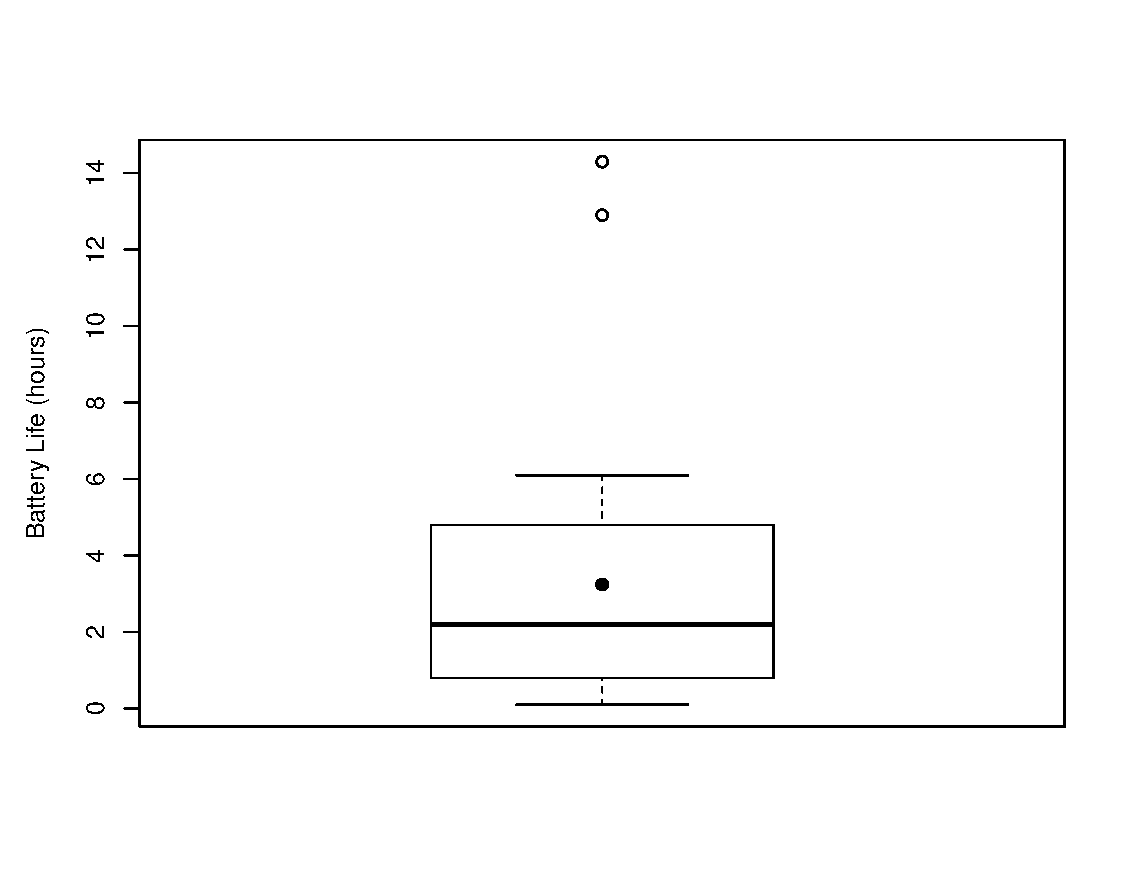
\includegraphics[width=0.8\textwidth, trim = 0.0cm 0.5cm 0.3cm 1cm, clip]{Boxplot}
\end{center}
\begin{itemize}\itemsep0.2cm
\item Boxplot without labels.
\end{itemize}

\end{frame}


\subsection{Boxplot Vs Histogram}
\begin{frame}{\bf \tcb{Boxplot Vs Histogram}\\[-1.1cm]}
\begin{center}
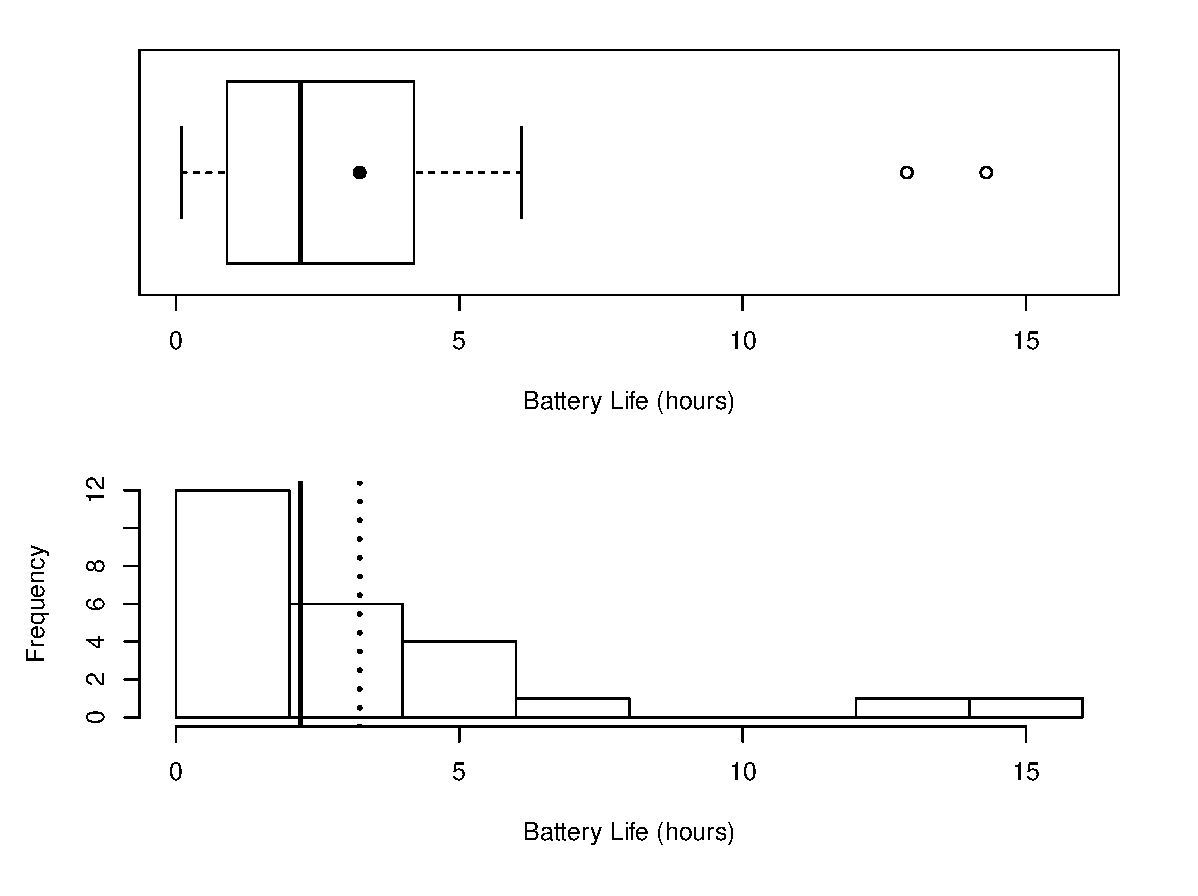
\includegraphics[width=0.86\textwidth, trim = 0.2cm 0.0cm 1cm 0.0cm, clip]{BoxplotHist}
\end{center}
\end{frame}






\subsection{Question 4}
\begin{frame}{\bf \tcb{Question 4}}
It turns out that the laptops can be split into two groups. The battery lives for each of the 25 laptops is shown below:\vspace{-0.2cm}
\begin{adjustwidth}{-0.3cm}{}
\begin{tabular}{|cccccccccccc|}
\hline
&&&&&&&&&&&\\[-0.4cm]
Type 1: & 0.1 & 0.2 & 0.2 & 0.4 & 0.7 & 0.9 & 1.0 & 1.5 & 2.3 & 4.2 & 5.6 \\[0.1cm]
\hline
&&&&&&&&&&&\\[-0.4cm]
Type 2: & 0.7 & 1.0 & 1.4 & 1.6 & 2.2 & 3.0 & 3.0 & 3.3 & 3.4 & 5.4 & 5.7 \\
& 6.1 & 12.9 & 14.3 &&&&&&&&\\
\hline
\end{tabular}
\end{adjustwidth}
\begin{enumerate}[a)]\itemsep0.3cm
\item Calculate the means for the two groups: $\bar x_1$ and $\bar x_2$.
\item What are the values of $n_1$ and $n_2$?
\item Draw the boxplots for each group (side by side on the same graph) and comment.
\item Are there outliers in either group?
\item Are either of the distributions skewed? If so, in what direction?
\end{enumerate}
\end{frame}



\section{Symbols}
\subsection{Recap of Symbols}
\begin{frame}{\bf \tcb{Recap of Symbols}}
Firstly, the sample size is $n$. The other symbols are given below:\\[0.3cm]
\begin{center}
\begin{tabular}{|c|c|c|}
\hline
&&\\[-0.3cm]
& Sample & Population \\
Quantity & Statistic & Parameter \\[0.1cm]
\hline
&&\\[-0.3cm]
Proportion & $\hat p$ & $p$ \\[0.2cm]
Mean & $\bar x$ & $\mu$ \\[0.2cm]
Variance & $s^2$ & $\sigma^2$ \\[0.2cm]
Standard Deviation & $s$\phantom{$^2$} & $\sigma$\phantom{$^2$} \\[0.2cm]
Quartiles & $Q_1$, $Q_2$, $Q_3$ & ---\\[0.2cm]
\hline
\multicolumn{3}{c}{}\\
\end{tabular}
\end{center}
{\footnotesize(we did not assign symbols to population quartiles)}
\end{frame}




\section{R Code}
\subsection{R Code: Centrality}
\begin{frame}{\bf \tcb{R Code: Centrality}}
The code used to calculate the mean and median for the income example is:\\[0.6cm]
\begin{tabular}{|l|}
\hline
\texttt{income = c(25, 29, 33, 35, 40)}\\
\texttt{mean(income)}\\
\texttt{median(income)}\\
\hline
\multicolumn{1}{c}{}\\[-0.1cm]
\end{tabular}

\end{frame}

\subsection{R Code: Dispersion}
\begin{frame}{\bf \tcb{R Code: Dispersion}}
The code used to calculate the variance and standard deviation for the income example is:\\[0.1cm]
\begin{tabular}{|l|}
\hline
\texttt{income = c(25, 29, 33, 35, 40)}\\
\texttt{var(income)}\\
\texttt{sd(income)}\\
\hline
\multicolumn{1}{c}{}\\[0.1cm]
\end{tabular}

Quartiles (as well as the minimum, maximum and mean) are given by the \texttt{summary} function:\\[0.1cm]
\begin{tabular}{|l|}
\hline
\texttt{x = c(2, 4, 2, 1, 5, 3, 0, 4, 1, 8)}\\
\texttt{summary(x)}\\
\hline
\multicolumn{1}{c}{}\\[-0.1cm]
\end{tabular}

R uses a slightly different method for calculating $Q_1$ and $Q_3$ to what we use in this course - so the results will be different to the lecture.\\[0.4cm]

Finally IQR is found via $\boxed{\text{\texttt{IQR(x)}}}$ - again different to the lecture.
\end{frame}


\subsection{R Code: Sort}
\begin{frame}{\bf \tcb{R Code: Sort}}
Another useful function is the \texttt{sort} function which orders the data from smallest to largest.\\[0.3cm]

\begin{tabular}{|l|}
\hline
\texttt{laptop = c(2.2, 0.4,  4.2, 12.9,  1.5,}\\
\hspace{2.5cm}\texttt{3.0,  5.7,  0.7,  1.0,  3.3,}\\
\hspace{2.5cm}\texttt{0.2,  0.2,  5.6,  1.6,  3.0,}\\
\hspace{2.5cm}\texttt{0.1, 14.3,  3.4,  0.9,  6.1,}\\
\hspace{2.5cm}\texttt{1.4,  1.0,  0.7,  5.4,  2.3)}\\
\texttt{laptop = sort(laptop)}\\
\texttt{laptop}\\
\hline
\multicolumn{1}{c}{}\\[-0.1cm]
\end{tabular}

\end{frame}



\subsection{R Code: Boxplot}
\begin{frame}{\bf \tcb{R Code: Boxplot}}
Using the \texttt{laptop} data from the previous slide, we can draw a boxplot (and include the mean) using\\[0.3cm]
\begin{tabular}{|l|}
\hline
\texttt{boxplot(laptop, xlab="Battery Life (hours)")}\\
\texttt{points(x=1,y=mean(laptop),pch=20)}\\
\hline
\multicolumn{1}{c}{}\\[-0.3cm]
\end{tabular}

{\footnotesize(Remember that R uses a different formula to get $Q_1$ and $Q_3$. So the boxplot will be slightly different to the one you do by hand)}\\[0.7cm]


A horizontal boxplot is given by\\[0.3cm]
\begin{tabular}{|l|}
\hline
\texttt{boxplot(laptop, horizontal=T, }\\
\hspace{2cm}\texttt{xlab="Battery Life (hours)")}\\
\texttt{points(x=mean(laptop),y=1,pch=20)}\\
\hline
\multicolumn{1}{c}{}\\[-0.1cm]
\end{tabular}
\end{frame}


\subsection{R Code: Two Boxplots}
\begin{frame}{\bf \tcb{R Code: Two Boxplots}}
Two boxplots side by side with mean values shown:\\[0.2cm]
\begin{tabular}{|l|}
\hline
\texttt{laptop1 = c(0.1, 0.2,  0.2, 0.4,  0.7, 0.9,  1.0,}\\
\hspace{2.8cm}\texttt{1.5, 2.3,  4.2, 5.6)}\\
\texttt{laptop2 = c(0.7, 1.0, 1.4, 1.6, 2.2, 3.0, 3.0,}\\
\hspace{2.8cm}\texttt{3.3, 3.4, 5.4, 5.7, 6.1, 12.9, 14.3)}\\[0.2cm]
\texttt{boxplot(laptop1,laptop2,}\\
\hspace{2.8cm}\texttt{xlab="Battery Life (hours)")}\\
\texttt{points(x=1,y=mean(laptop1),pch=20)}\\
\texttt{points(x=2,y=mean(laptop2),pch=20)}\\
\hline
\multicolumn{1}{c}{}\\[-0.1cm]
\end{tabular}

\end{frame}




\end{document} 